Для установки оперционной системмы Raspbian на Raspberry Pi необходимо перейти на страницу загрузок на официальном сайте~\cite{raspbian_downloads} и скачать необходимый образ ОС (рис.~\ref{raspbian_1:raspbian_1}), затем установить загруженный образ на SD-карту, которая впоследствии будет подключена к Raspberry Pi и с которой непосредственно будет загружаться система.

\begin{figure}[h!]
\center{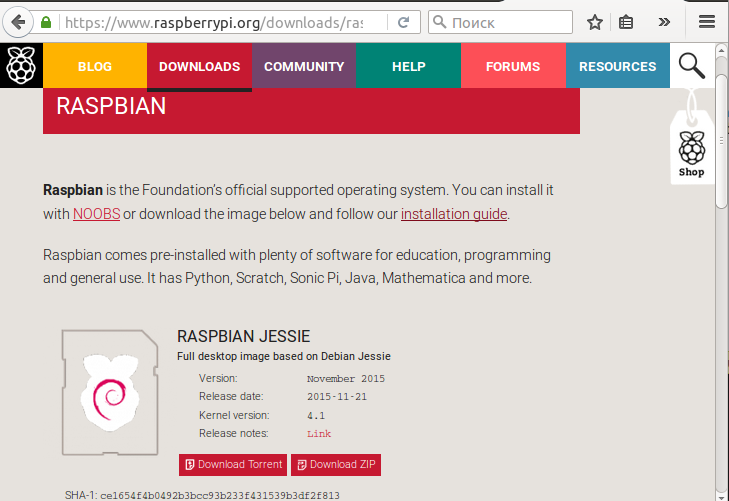
\includegraphics[width=0.8\linewidth]{raspbian_1}}
\caption{ Официальная страница загрузок ОС Raspbian }
\label{raspbian_1:raspbian_1}
\end{figure}

Инструкцию по установке образа системы на SD-карту можно найти, перейдя по ссылке~\cite{raspbian_install}. 

После распаковки заргуженного архива с образом системы, необходимо вставить SD-карту в слот и выполнить следующие команды:

\begin{verbatim}
$ df -h   # увидеть все примонтированные устройства 
$ umount /dev/<ИМЯ_УСТРОЙСТВА>    # отмонтировать SD-карту
$ dd bs=4M if=2015-11-21-raspbian-jessie.img of=/dev/sdd    # записать образ
$ sync
\end{verbatim}

Далее достаточно извлечь SD-карту и установить ее в соответсвующий разъем Raspberry Pi.
